\documentclass[12pt]{article}
\textwidth=7in
\textheight=9.5in
\topmargin=-1in
\headheight=0in
\headsep=.5in
\hoffset  -.85in

\pagestyle{empty}

\usepackage{amsmath,amssymb,amsfonts}
\usepackage{url}
\usepackage{graphicx}

\renewcommand{\thefootnote}{\fnsymbol{footnote}}
\begin{document}

\begin{center}
{\bf Introduction to Data Science \\ Homework 2: Due Wednesday September 5 at 2:00pm}
\end{center}

\setlength{\unitlength}{1in}

\begin{picture}(6,.1)
\put(0,0) {\line(1,0){6.5}}
\end{picture}

\renewcommand{\arraystretch}{2}

\vskip.25in

\noindent{\bf  {\Large Exercises:} }

\vskip.25in
  \begin{enumerate}
    \item   Read the Structured Data handout and the first few sections through \emph{Visualising distributions} of \emph{R for Data Science}. 
    \item Find a data set or data sets that exemplify each of the terms: rectangular or tabular data, continuous, discrete, categorical, binary, ordinal.
    \item Explain why it is important to have a taxonomy of data types. 
    \item True or False: The {\tt diamonds} data set in the {\tt ggplot2} package is a data frame. One way to answer this question is by typing the command {\tt str(diamonds)} in R. 
    \item True or False: The {\tt diamonds} data set in the {\tt ggplot2} package is ``tidy.''
    \item How many variables are there in the {\tt diamonds} data set?
    \item Classify each of the variables in the {\tt diamonds} data set. That is, state if the variable is continuous, discrete, categorical, etc. 
    \item Describe the difference between a bar plot and a histogram. Under what circumstances would you use each? 
    \item Explain the result of the command 
    \begin{verbatim}
      ggplot(data = mpg) + geom_bar(mapping = aes(x=class))
    \end{verbatim}
    You should get a plot that looks like this:
    \begin{figure}[htbp]
        \begin{center}
           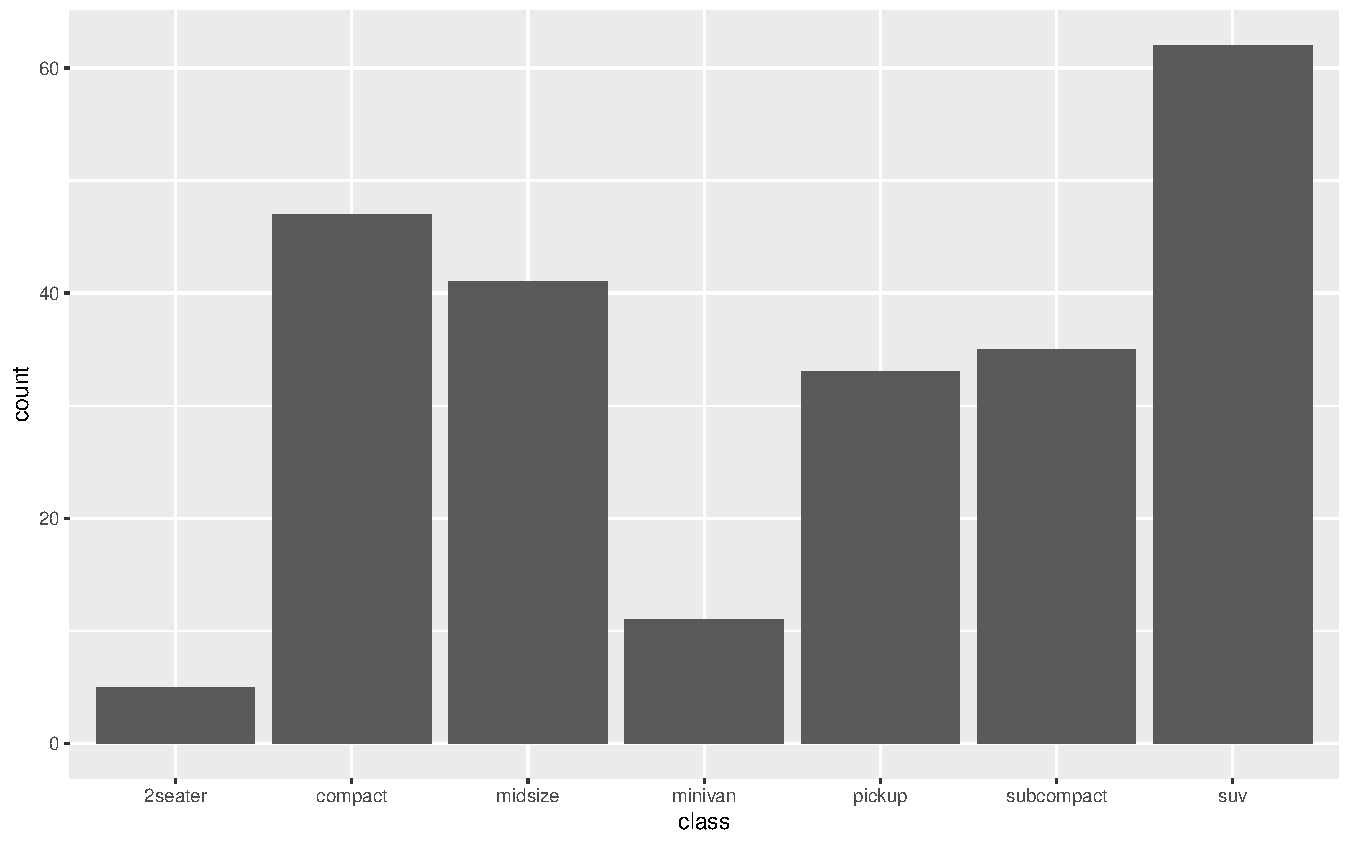
\includegraphics[scale=0.4]{exampleBar.pdf}
        \end{center}
    \end{figure}
    
 Make sure to answer the question in the context of the data. 
  \item Explain the result of the command 
    \begin{verbatim}
      ggplot(data = mpg) + geom_histogram(mapping = aes(x=displ),binwidth=0.4)
    \end{verbatim}
    You should get a plot that looks like this:
    \begin{figure}[htbp]
        \begin{center}
           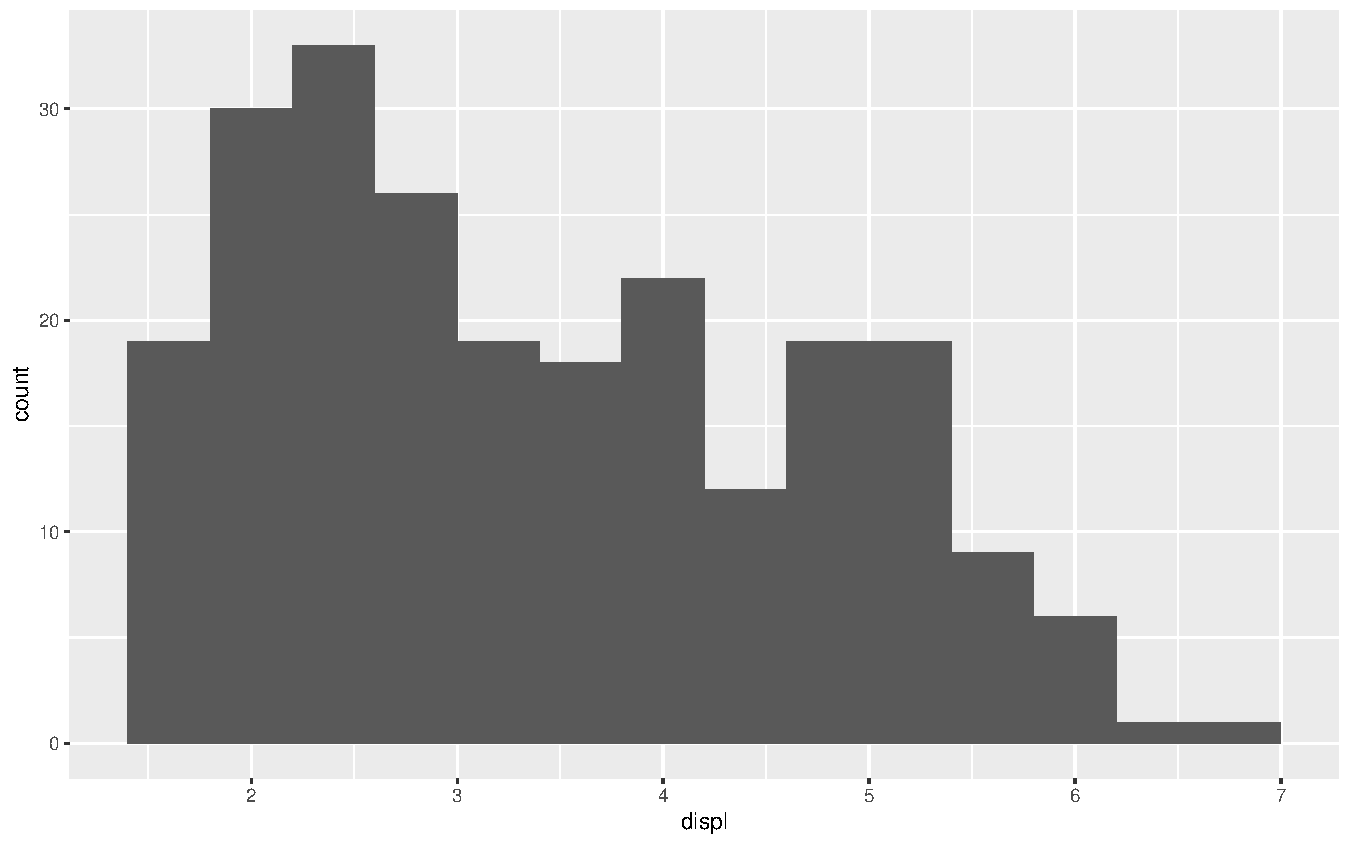
\includegraphics[scale=0.4]{exampleHist.pdf}
        \end{center}
    \end{figure}
    
 Make sure to answer the question in the context of the data. 
  \end{enumerate}
\end{document}
